\chapter{System Evaluation} \label{eval}
As discussed in section \textit{1.1: Project Objectives}, we will now expand on the system implemented in this project.

\paragraph{Dissertation}
\begin{itemize}
\item Introduce the concept of the project. 
\item Provide an understanding of social media.
\item Provide a understanding of web technologies.
\item Describe the development of the applied project
\end{itemize}
 
 \paragraph{Applied Project}
\begin{itemize}
\item Produce a simple easy to use web application.
\item Deliver a social platform for tech savvy people that differs from the norm.
\item Dive into new web technologies.
\item Complete the project collaborating as a team using an efficient and effective approach.
\end{itemize}

% ========================== Testing ========================== 
\section{Testing}
It was an important part of the project for us to plan out the project, and test each component of the full stack web-development. We started prototyping the MEAN stack as well as developing the project early to test the functionality early.

\subsection{Prototyping}
Early on we built multiple applications to test the functionality of the MEAN stack. We built a Node.js application, then added ExpressJS. Getting a basic grasp of each technology before advancing was very import as to understanding how the system as a whole will work from top to bottom.

\begin{figure}[H]
  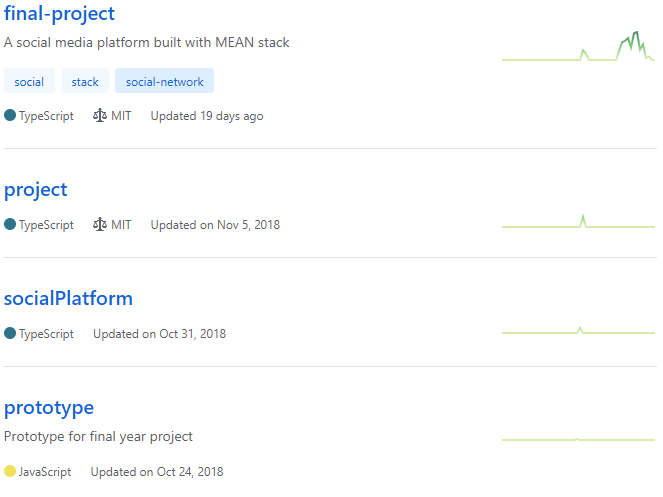
\includegraphics[width=\linewidth]{img/prototypes.PNG}
  \caption{GitHub Prototypes}
  \label{fig:GHP}
\end{figure}

As you can see above there is four GitHub projects. The first one at the top is the final project. The rest are prototypes we developed to test the MEAN stack functionality and understand each component of the MEAN stack (MongoDB, ExpressJS, Node.js and Angular).

\subsection{Deployment Testing}
We tested the project using a three stage deployment. Initial, medial and final. Each stage covered a criteria on the deployment process. Initial used for unit testing, medial for early deployment testing and final for the public release of the application.

\subsubsection{Initial}
Initial testing involved testing the application on the local-host and test each functionality to see how the application would react to our inputs. This was the primary method of testing individual components and ensuring the application would work on the local-host port 3000.

\subsubsection{Medial}
After the initial testing stage we had a medial stage for deployment. We built a home server to test the application over a network. This involved buying and building the home server. Once setup and built we connected the PC to the home network and gave the PC a static IP (Internet Protocol). This was extremely important, without giving the server a static IP the local address such as 192.168.0.10 could be moved to 192.168.0.50. If the local IP of the server changed, the port forwarding address would need to change each time the server's did, which would be very tedious. 

Once the IP of the server was setup we port forwarded the port 3000 to the server PC's static IP address. The port 3000 had to be port forwarded because of the application using that port. With this setup we could access the application from another PC in another location. This was used to demo the application to supervisors in meetings.

\subsubsection{Final}
With a grasp on how deployment works from the stage above we had the knowledge on how and what needed to be done. We deployed our project on AWS (Amazon Web Services). We went with AWS because of their support for the MEAN stack made it a prime contender. Once deployed onto AWS we knew we could access it from inside the instance, but not outside. So knew from above we need to open the port and direct it to our AWS instance. Although in this case, AWS handled the local IP and all we had to do in deployment in this stage was open the port using AWS console, which acted as a router for our AWS instance.

\subsection{Unit Testing}
testing parts of program


% ========================== Performance ========================== 
\section{Performance}
Use performance benchmarks (space and time) if algorithmic.

% ========================== Objectives ========================== 
\section{Evaluation of Objectives}
Measure the outcomes / outputs of your system / software against the objectives from the Introduction.
\subsection{Objective 1}
did we reach our objective?

\subsection{Objective 2}
did we reach our objective?

\subsection{Objective 3}
did we reach our objective?

\subsection{Objective 4}
did we reach our objective?

% ========================== Limitations ========================== 
\section{Limitations}
Areas for improvement?
Highlight any limitations or opportuni-ties in your approach or technologies used.